%-------------------------------------------------------------------------
% Aulia Kharis Rakhmasari — CV
% Compiles with pdfLaTeX on Overleaf. No exotic packages.
%-------------------------------------------------------------------------
\documentclass[10.5pt,a4paper]{article}

\usepackage{charter}
\usepackage[T1]{fontenc}
\usepackage[utf8]{inputenc}
\usepackage[margin=1.6cm,top=1.4cm,bottom=1.4cm]{geometry}
\usepackage{graphicx}
\usepackage{enumitem}
\usepackage{titlesec}
\usepackage{xcolor}
\usepackage[hidelinks]{hyperref}
\usepackage{tabularx}

% ---- colours -------------------------------------------------------------
\definecolor{accent}{HTML}{1F3A5F}
\definecolor{rule}{HTML}{B9C2CC}

% ---- section formatting --------------------------------------------------
\titleformat{\section}
  {\normalfont\large\bfseries\color{accent}}{}{0em}{}[\vspace{-0.55em}\color{rule}\rule{\linewidth}{0.8pt}]
\titlespacing*{\section}{0pt}{1.0em}{0.45em}

% ---- helpers -------------------------------------------------------------
\newcommand{\entry}[4]{%
  \noindent\begin{tabularx}{\linewidth}{@{}Xr@{}}
    \textbf{#1} & \textbf{#3} \\
    \textit{#2} & \textit{#4} \\
  \end{tabularx}\vspace{0.15em}
}

\newenvironment{bullets}
  {\begin{itemize}[leftmargin=1.1em,itemsep=0.12em,topsep=0.18em,parsep=0pt]}
  {\end{itemize}}

\setlength{\parindent}{0pt}
\pagestyle{empty}

%==========================================================================
\begin{document}

% \noindent
% \begin{minipage}[c]{0.74\linewidth}
%   {\LARGE\bfseries\color{accent} Aulia Kharis Rakhmasari}\\[0.4em]
%   {\small MSc Data Science, ETH Zürich}\\[0.3em]
%   {\small arakhmasari@ethz.ch \ $\cdot$ \ +41 76 829 56 82 \ $\cdot$ \ Zürich, CH}\\[0.15em]
%   {\small \href{https://github.com/auliakharis}{github.com/auliakharis} \ $\cdot$ \ \href{https://www.linkedin.com/in/aulia-kharis-rakhmasari/}{LinkedIn}}
% \end{minipage}\hfill
% \begin{minipage}[c]{0.22\linewidth}
%   \raggedleft
%   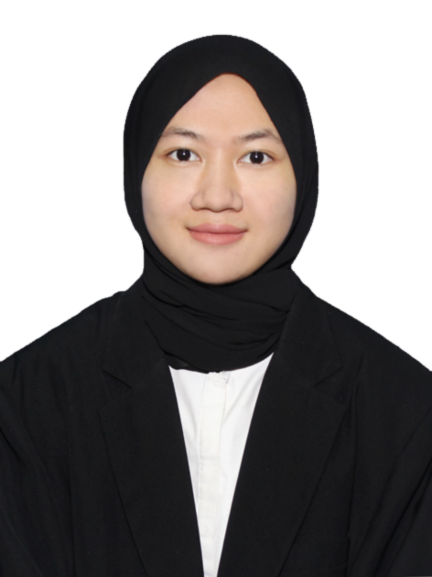
\includegraphics[height=3.4cm,keepaspectratio]{foto_formal_aulia.png}
% \end{minipage}
% \vspace{0.8em}

% ---------------------------- HEADER -------------------------------------
\begin{center}
  {\LARGE\bfseries\color{accent} Aulia Kharis Rakhmasari}\\[0.35em]
  {\small
    Zürich, Switzerland \quad\textbar\quad +41 76 829 56 82 \quad\textbar\quad
    \href{mailto:arakhmasari@ethz.ch}{arakhmasari@ethz.ch}\\[0.2em]
    \href{https://github.com/auliakharis}{github.com/auliakharis} \quad\textbar\quad
    \href{https://www.linkedin.com/in/aulia-kharis-rakhmasari/}{linkedin.com/in/aulia-kharis-rakhmasari}
  }
\end{center}
\vspace{-0.3em}

% ---------------------------- SUMMARY ------------------------------------
\section{Profile}
MSc Data Science candidate at ETH Zürich working on LLM evaluation and alignment for regulated
domains: LLM-as-a-Judge methodology, preference optimisation (DPO/LoRA), and benchmark design for
financial and legal NLP. Previously 2 years as a production Data Scientist in banking,
shipping ML pipelines with measurable revenue impact.
% TODO: adjust the authorship claim above if either paper is not first-author.

% ------------------------ SKILLS -----------------------------------------
\section{Technical Skills}
\begin{tabularx}{\linewidth}{@{}p{3.1cm}X@{}}
  \textbf{ML \& LLMs}    & PyTorch, Hugging Face (Transformers, PEFT, TRL), LoRA, DPO/RLHF,
                           LLM-as-a-Judge evaluation, benchmark design, VLMs, TensorFlow \\[0.25em]
  \textbf{Infrastructure}& SLURM / Euler HPC, Git, Bash, Cloudera Data Science Workbench \\[0.25em]
  \textbf{Languages}     & Python, R, SQL, C++\\[0.25em]
  \textbf{Data \& BI}    & Advanced SQL at scale, Power BI, Tableau, R Shiny, Excel/VBA \\
\end{tabularx}


% ---------------------------- EDUCATION ----------------------------------
\section{Education}

\entry{ETH Zürich}{MSc Data Science, DINFK}{Zürich, Switzerland}{Sep 2025 -- expected Sep 2027}
\begin{bullets}
    \item Teaching Assistant for Python and Machine Learning : D-ITET
  \item Fully funded by the Indonesian Government (LPDP) scholarship; acceptance rate $<5\%$.
  \item Coursework: Deep Learning, Probabilistic AI, Machine Learning in Finance,
        Algorithmic Foundations of Data Science, Computational Statistics.
\end{bullets}

\entry{Institut Teknologi Sepuluh Nopember (ITS)}{BSc Statistics --- GPA 3.97/4.00}{Surabaya, Indonesia}{Jul 2019 -- Jul 2023}
\begin{bullets}
  \item \textbf{Best Graduate} among 1{,}000+ graduates; highest GPA in the 2019 cohort.
  \item Fully funded AIG Insurance Science Scholarship (semesters 3--8).
  \item Thesis: Marked Log-Gaussian Cox Process for estimating household expenditure per capita,
        Central Java. 
\end{bullets}

\entry{Uniwersytet Szczeciński}{Exchange semester, Economics and Management}{Szczecin, Poland}{Sep 2021 -- Feb 2022}
\begin{bullets}
  \item Fully funded by the European Union under Erasmus+ International Credit Mobility.
\end{bullets}

% ------------------------ PUBLICATIONS -----------------------------------
\section{Publications \& Peer Review}
\begin{bullets}
  \item \textbf{V-FiLLM: Verified Financial LLM Reasoning Benchmark}
        \hfill {\small\href{https://arxiv.org/abs/2608.11047}{arXiv:2608.11047}}
  \item \textbf{FinRegQA-EU: Corruption-Based Preference Data for Grounded EU Financial Regulatory Question Answering}
        \hfill {\small\href{https://arxiv.org/abs/2609.36856}{arXiv:2608.11047}}

  \item \textbf{Investigating Relational Reasoning in VLMs}
        \hfill {\small\href{https://arxiv.org/abs/2608.23518}{arXiv:2608.23518}}
  \item \textbf{Reviewer}, FinNLP @ EMNLP 2026.
\end{bullets}

% ------------------------ RESEARCH ---------------------------------------
\section{Research Experience}

\entry{FinRegQA-EU: Corruption-Based Preference Data for Grounded EU Financial Regulatory Question Answering}{Law, Economics and Data Science Group (Prof.\ Elliott Ash), ETH Zürich}{}{2026}
\begin{bullets}
  \item Built an end-to-end evaluation and alignment pipeline on ETH's Euler HPC
        cluster over a purpose-built EBA/ESMA regulatory Q\&A dataset.
  \item Ran multi-judge LLM-as-a-Judge evaluation across three judge models
        (Gemma-4-31B, Qwen3.5-27B, GLM-4.7-Flash); measured inter-judge agreement and found
        near-zero Krippendorff's $\alpha$ on citation quality despite strong agreement on accuracy.
  \item Fine-tuned Qwen3.5-4B with DPO across five preference-corruption strategies and introduced a
        \textbf{Citation F1} metric; showed that LLM judges are systematically blind to citation
        improvements that Citation F1 captures.
\end{bullets}

\entry{V-FiLLM --- Verifiable Financial Reasoning Benchmark}{ETH AI Center $\times$ Apertus (supervisor: Dr.\ Nino Antulov-Fantulin)}{}{2026}
\begin{bullets}
  \item Designed a deterministic computation-tree benchmark generating financial reasoning tasks
        with verifiable ground truth over structured tabular data.
  \item Benchmarked eight open and frontier models (incl.\ Apertus-70B, Llama-3.3-70B, Qwen3.5-27B)
        and ran LoRA fine-tuning experiments to quantify achievable gains.
  \item Stress-tested robustness under adversarial perturbations: missing values, OCR lookalike
        substitutions, prompt injection, and cross-table contamination.
\end{bullets}

\entry{Gated Graph-of-Gradients DPO --- Fairness in LLM Alignment}{ETH AI Center}{}{2026}
\begin{bullets}
  \item Investigated whether DPO loss disparities track demographic groups using the PRISM dataset.
  \item Showed that demographic grouping does \textit{not} explain loss variation, whereas
        gradient-space grouping does; built a graph-of-gradients reweighting method on that finding.
\end{bullets}

\entry{Relational Reasoning in Vision-Language Models}{ETH Zürich --- completed}{}{Sep 2025 -- Jan 2026}
\begin{bullets}
  \item Evaluated state-of-the-art VLMs on spatial, semantic, and compositional relational tasks;
        identified failure modes and proposed targeted evaluation benchmarks.
\end{bullets}

\entry{Research Assistant --- Spatial Statistics}{Institut Teknologi Sepuluh Nopember}{}{Jun 2022 -- Jun 2023}
\begin{bullets}
  \item Marked LGCP modelling in R under Dr.\ A. Choiruddin, Dr.\ Sutikno, and Prof.\ J. Mateu
        (Universitat Jaume I)
\end{bullets}

% ------------------------ INDUSTRY ---------------------------------------
\section{Industry Experience}

\entry{Data Scientist (full-time)}{Bank Syariah Indonesia}{Jakarta, Indonesia}{Sep 2023 -- Sep 2025}
\begin{bullets}
  \item Built and automated end-to-end ML pipelines in Python (Cloudera CDSW) for credit
        card programmes supporting over CHF~28M in annual card spend.
  \item Developed propensity models to reactivate dormant users and onboard new-to-bank
        customers, generating 
        CHF~ 1.7 M+ in incremental transaction volume.
  \item Shipped an automated Next Best Offer recommendation engine for monthly personalised targeting.
  \item Forecast ATM and teller traffic through peak season at $<5\%$ MAPE, integrated into live dashboards.
\end{bullets}
% NOTE: IDR figures converted at ~1 CHF = 17,800 IDR. Verify before sending, and keep the original
% IDR in brackets if applying to Indonesian or regional employers.

\entry{Data Scientist (part-time)}{Siena Clinical}{Jakarta, Indonesia (remote)}{May 2024 -- Present}
\begin{bullets}
  \item Built an interactive meta-analysis web application in R Shiny for real-time clinical
        data visualisation.
  \item Analysed clinical datasets for a study classifying benign prostatic hyperplasia
        vs.\ carcinoma; delivered internal training on meta-analysis in R.
\end{bullets}

\entry{Claim Data Analyst Intern}{AIG Insurance}{Jakarta, Indonesia}{May 2023 -- Aug 2023}
\begin{bullets}
  \item Automated claim reporting via Power BI dashboards and Excel VBA tooling; supported
        risk assessment on incoming claims.
\end{bullets}

\entry{Data Audit Analytics Intern}{PT XL Axiata Tbk}{Jakarta, Indonesia}{Feb 2022 -- Jun 2022}
\begin{bullets}
  \item Built KPI monitoring dashboards and presented audit findings on retail outlet and
        field survey data to senior management.
\end{bullets}

 
% ------------------------ AWARDS -----------------------------------------
\section{Selected Awards \& Honours}
\begin{bullets}
  \item \textbf{1st place}, TrackAML Hackathon, PPATK (Indonesian Financial Transaction
        Reports and Analysis Centre). \hfill 2023
  \item \textbf{Distinction Graduate}, Bangkit Academy (Google, GoTo, Traveloka) ---
        top 10\% of 4{,}500+ participants, machine learning track. \hfill 2023
  \item \textbf{AWS Datathon Side Challenge}, ETH Zürich. \hfill 2026
  \item \textbf{Gold Medal}, ASEAN Innovative Science \& Environmental Entrepreneur Fair;
        \textbf{Silver Medal}, World Science Environment \& Engineering Competition. \hfill 2021--2022
  \item \textbf{Fully funded scholarships:} LPDP (Indonesian Government, ETH MSc);
        Erasmus+ International Credit Mobility (EU); AIG Insurance Science Scholarship.
\end{bullets}

% ------------------------ ADDITIONAL -------------------------------------
\section{Additional}
\begin{bullets}
  % \item \textbf{Work authorisation:} ETH Zürich student --- eligible for up to 15 hours working per week. % TODO: confirm exact wording with ETH Career Services
  \item \textbf{Languages:} Indonesian (native), English (fluent, C1), German (A2).
  \item \textbf{Community:} Member, Data Science Indonesia (2021--present);
        President, Statistics Computer Course, ITS (2022).
\end{bullets}

\end{document}